\subsection{The Greedy Algorithm}
\label{greedy}
The results in the previous section concentrated on producing nearly
optimal solutions in expectation. In this section, we will show that
it is possible to obtain good solutions regardless of the model that
generated the recommendation subgraph. As usual we let $G=(L,R,E)$ be a
bipartite graph on which we would like to solve the $(c,a)$-graph
recommendation problem. 

We analyze the following natural greedy algorithm. Consider each vertex in $R$ in some arbitrary order and if there is some $v \in R$ that has $a$ neighbors in $L$ all of which have degree $< c$, add the edges to these neighbors to $H$. If there
are any ties about the nodes to be picked either in the selection of
$v$ or its neighbors, we can break ties arbitrarily. 

\begin{thm}
The greedy algorithm achieves a $1/(a+1)$-approximation ratio for the $(c,a)$-graph
recommendation problem.
\end{thm}
\begin{proof}
Let $R_{GREEDY}, R_{OPT}\subseteq R$ be the set of vertices that have
degree $\geq a$ in the greedy and optimal solutions respectively. Note
that any $v \in R_{OPT}$ along with neighbors $\{u_1,\ldots u_a\}$
forms a set of candidate edges that can be taken by the greedy
algorithm. So we can consider $R_{OPT}$ as a candidate pool for
$R_{GREEDY}$. Each move that the greedy algorithm makes might make
some of the candidates infeasible, but as long as the candidate pool
is not depleted, the greedy algorithm can continue adding vertices to
its solution. Each time the greedy algorithm claims some vertex $v\in
R$ with edges to $\{u_1,\ldots, u_a\}$, we have obviously have to
remove $v$ from the candidate pool. If any $u_i$ was saturated
(i.e. had degree $c$) in the optimal solution, we would also need to
remove an arbitrary vertex $v_i\in R$ adjacent to $u_i$ in the optimal
solution. In other words, by using an edge of $u_i$, we force it to
not use an edge it used to some other $v_i$, which might cause the
degree of $v_i$ to go below $a$. (Note that the greedy algorithm does
not actually have to be aware of the structure of optimal solution for
this type of bookkeeping to go through.) Therefore, at each step of
the greedy algorithm, we have to remove at most $a+1$ vertices from
the candidate pool. Since our candidate pool has size $OPT$, the
greedy algorithm cannot stop before it has added $OPT/(a+1)$
vertices to the solution.
\end{proof}

\begin{figure}[h]
\centering
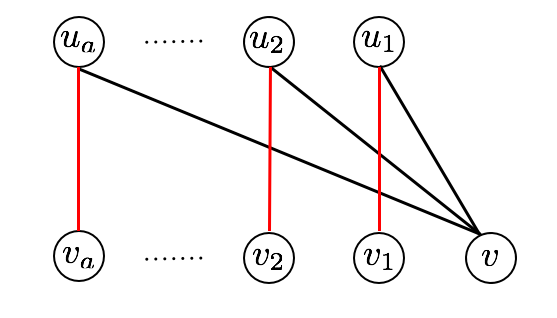
\includegraphics[width=.5\textwidth]{greedy.png}
\begin{minipage}[h]{.8\linewidth}
\caption{This diagram shows one step of the greedy algorithm. When $v$ claims edges to $u_1,\ldots, u_a$, it potentially removes $v_1,\ldots, v_a$ from the pool of candidates that are avaiable. The potentially invalidated edges are shown in red.}
\end{minipage}
\end{figure}

There are two things to note about this algorithm. The first is
that the solution the greedy algorithm outputs is dependent on the
order the vertices in $R$ are processed. It may be possible to improve
the expected approximation ratio by permuting these vertices randomly
before the algorithm runs. The second is that this approximation
guarantee is as good as we can expect. In particular, if we set $a=1$
then we obtain the familiar $1/2$-approximation of the greedy
algorithm for matchings.

%However, in reality, this algorithm fares much better when we put give it the same expectation treatment we have given the sampling algorithm.

Similar to the case with matchings, it's not hard to see that this
approximation ratio is tight for the greedy algorithm. Suppose, that
there are $a+1$ vertices $v_1,\ldots,v_{a+1}$ in $R$ and $(a+1)a$ 
vertices $u_{i,j}$ for $1\leq i\leq a+1$ and $1\leq j \leq a$ in $L$.
We add an edge between $u_{i,j}$ and $v_{i}$ for each $i$ and $j$.
We also add edges between $v_1$ and every other vertex. The optimal
$(1,a)$-recommendation subgraph simply matches each $v_i$ to each
$u_{i,j}$, and has size $a+1$. However, the greedy algorithm
could match $v_1$ to $u_{i,1}$ for each $2\leq i\leq a+1$, producing
a solution of size $a+1$. As in matchings, randomizing the order in
which the vertices are processed still leaves a constant factor gap
in the size of the solution as in the matchings case.
\cite{KarpVaziraniVazirani1990}

%Arda: Please add the description here of the example with L1, L2, R1, R2 with all edges except between L2 and R2 and the greedy edges preferring the neighbors in L having OPT=n but even a random permutation loses a constant factor. The online matching paper by Karp, Vazirani & Vazirani has som eversion of this example - Cite if it is relevant: there is a more recent Birnbaum-Mathieu reference of this result.

\begin{thm}
Let $G=(L,R,E)$ be a graph drawn from the $G_{l,r,p}$. If $S$ is the size of the $(c,a)$-recommendation subgraph produced by the greedy algorithm, then:
\[ \E[S] \geq r - \frac{a(lp)^{a-1}}{p}\]
\end{thm}
\begin{proof}
Note that if edges are generated uniformly, then we can consider the
graph as being revealed to us one vertex at a time as the greedy
algorithm runs. In particular, consider the event $X_i$ that the
greedy algorithm matches the $(i+1)^{th}$ vertex it inspects. While,
$X_{i+1}$ is dependent on $X_1,\ldots, X_i$, the worst condition for
$X_{i+1}$ is when all the previous $i$ vertices were by the same
vertices in $L$, which are now not available for matching the
$(i+1)^{th}$ vertex. The maximum number of such invalidated vertices
is at most $\lceil i/c \rceil$. Therefore, the probability that fewer
than $a$ of the of the at least $l-\lceil i/c \rceil $ available 
vertices have an edge to this vertex is at most $\Pr[Y\sim (l-i/c,p): Y < a]$.
Using the crude approximation that
\[ \Pr[Y\sim Bin(l-ia/c,p): Y < a] \leq a(1-p)^{l-ia/c-a}(lp)^{a-1}\]
and summing over all the $X_i$ using the linearity of expectation,
we obtain the following inequality:

\begin{align*}
      \E[S]
&\geq r - \sum_{i=0}^{r-1} \E[\lnot X_i] \\
&\geq r - \sum_{i=0}^{r-1} \Pr[Y \sim Bin(l-ia/c,p): Y < a] \\
&\geq r - \sum_{i=0}^{r-1}a(1-p)^{l-ia/c-a}((l-ia/c)p)^{r-1} \\
&\geq r - a(lp)^{r-1}\sum_{i=0}^{r-1}(1-p)^{l-ia/c-a} \geq r - \frac{a(lp)^{a-1}}{p}\\
\end{align*}
\end{proof} 
